\section{Recursively bisecting meshes [15 points]}
In this exercise we recursively partition 2D graphs derived by structural engineering matrices provided by Nasa. For that we use the provided function \texttt{Recursion}, which takes a bisection algorithm and graph as arguments and then partitions the graph into $2^l$ subpartitions. In our case we chose $l$ to be 3 and 4 to create 8 and 16 partitions respectively. The resulting edge-cuts for both partition sizes can be found in table \ref{tab:rec_bi_combined}.
%TODO: Interpretation
Furthermore an example for the visual result of different algorithms for the mesh \texttt{crack} using 16 partitions can be seen in Figure \ref{fig:rec_bi}.
\begin{table}[H]
	\centering
	\resizebox{\textwidth}{!}{ % This scales the table to fit the page width
	\begin{tabular}{lcccccccc}
		\toprule
		\multirow{2}{*}{Mesh} & \multicolumn{4}{c}{Edge Cut (8 Partitions)} & \multicolumn{4}{c}{Edge Cut (16 Partitions)} \\
		\cmidrule(lr){2-5} \cmidrule(lr){6-9}
		                     & Coordinate & Metis 5.0.2 & Spectral & Inertial & Coordinate & Metis 5.0.2 & Spectral & Inertial \\
		\midrule
		airfoil1             & 397        & 318         & 516      & 670      & 629        & 516         & 819      & 1081     \\
		netz4504\_dual       & 112        & 96          & 127      & 165      & 183        & 159         & 198      & 271      \\
		stufe                & 129        & 108         & 123      & 320      & 246        & 193         & 227      & 606      \\
		3elt                 & 469        & 418         & 733      & 814      & 752        & 699         & 1168     & 1230     \\
		barth4               & 549        & 470         & 875      & 977      & 549        & 470         & 875      & 1492     \\
		ukerbe1              & 781        & 147         & 225      & 340      & 888        & 245         & 374      & 499      \\
		crack                & 883        & 808         & 1343     & 1351     & 1419       & 1275        & 1860     & 1884     \\
		\bottomrule
	\end{tabular}
	}
	\caption{Edge cut results for recursive bi-partitioning using 8 and 16 partitions.}
	\label{tab:rec_bi_combined}
\end{table}



\begin{figure}[H]
	\centering
	\begin{subfigure}{0.5\textwidth}
		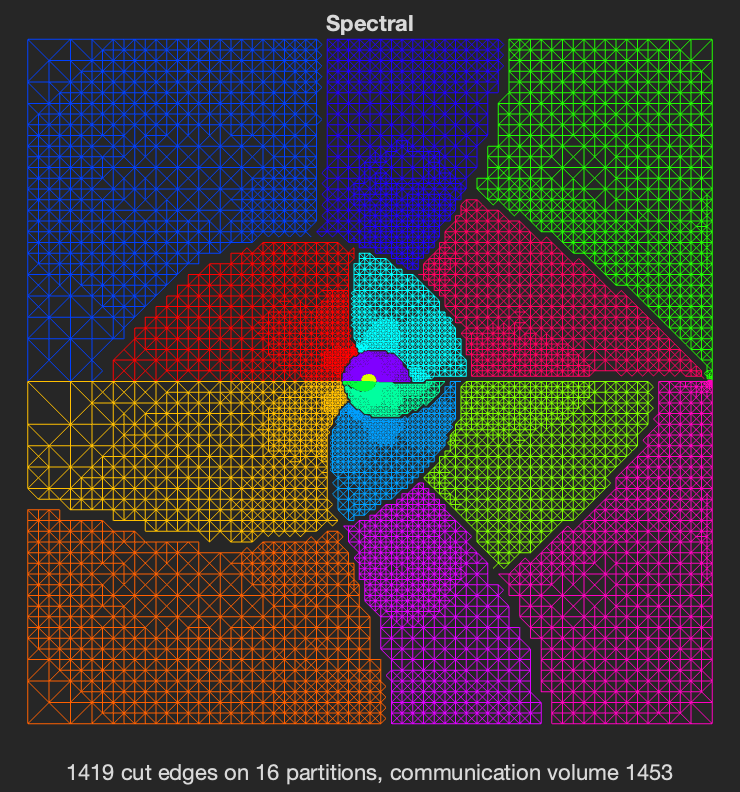
\includegraphics[width=\textwidth]{./media/spec_crack.png}
		\caption{Spectral bisection}
		\label{fig:spec_crack}
	\end{subfigure}%
    ~
	\begin{subfigure}{0.5\textwidth}
		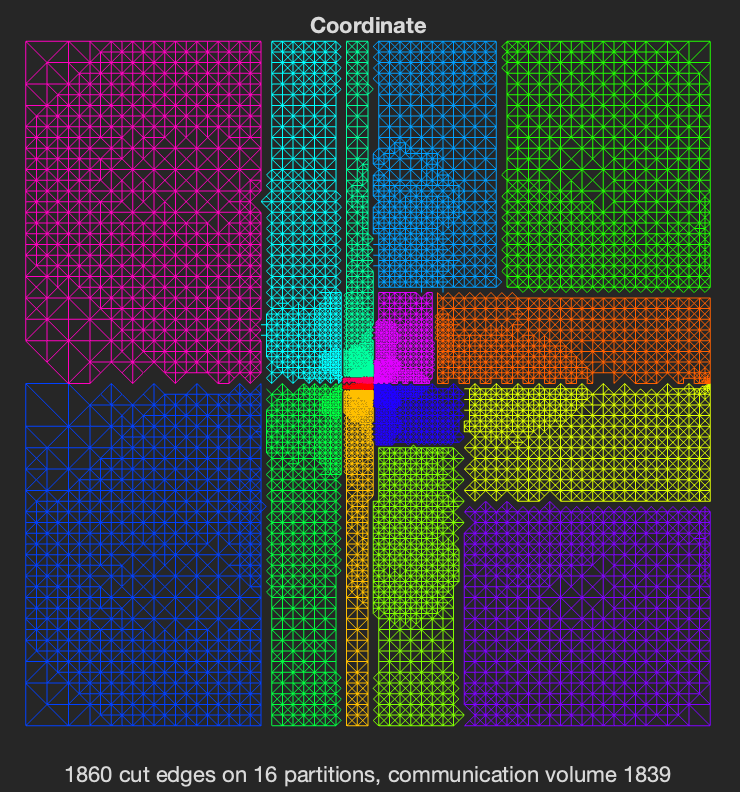
\includegraphics[width=\textwidth]{./media/coord_crack.png}
		\caption{Coordinates bisection}
		\label{fig:coord_crack}
	\end{subfigure}\\
	\begin{subfigure}{0.5\textwidth}
		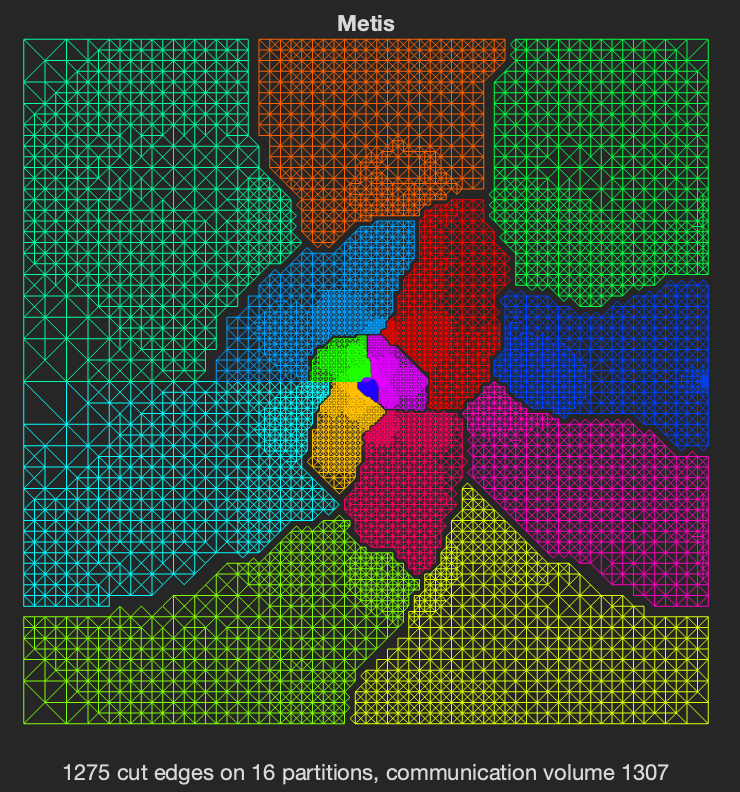
\includegraphics[width=\textwidth]{./media/metis_crack.png}
		\caption{Metis bisection}
		\label{fig:metis_crack}
	\end{subfigure}%
    ~
	\begin{subfigure}{0.5\textwidth}
		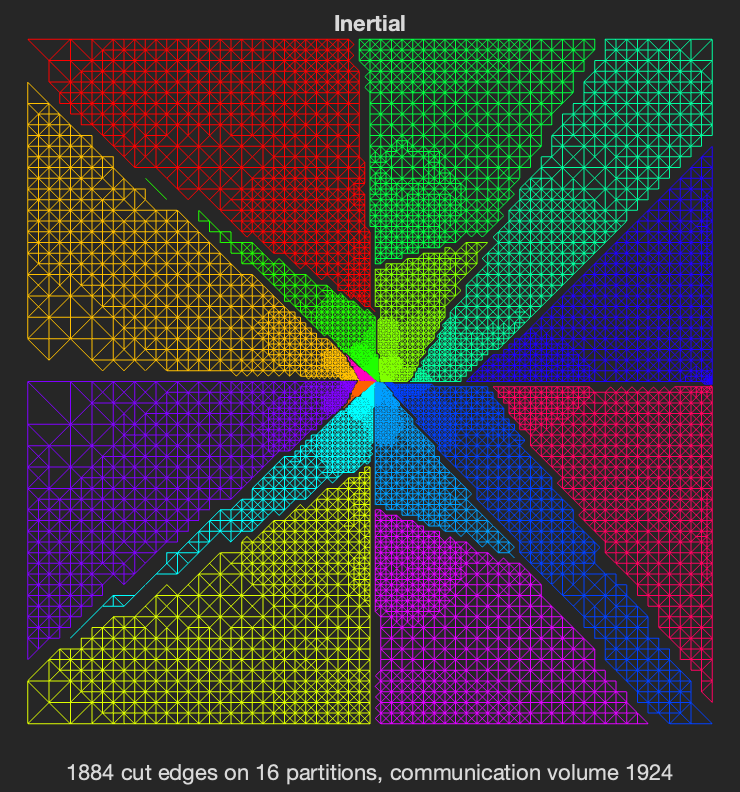
\includegraphics[width=\textwidth]{./media/inert_crack.png}
		\caption{Inertial Bisection}
		\label{fig:inert_crack}
	\end{subfigure}
	\caption{Recursive bisecting of mesh "crack" into 16 partitions with different algorithms.}
	\label{fig:rec_bi}
\end{figure}

